\documentclass{beamer}
\usepackage[utf8]{inputenc}
\usepackage{caption}
\usetheme{Warsaw}


%Information to be included in the title page:
\title{DRASIL}
\subtitle{A Knowledge-Based Approach to Scientific Software Development}
\author{Henry M, Aaron M, Maryyam N, Nicholas R, Dan S}
\institute{McMaster University}
\date[LSS \today]{Literate Scientific Software Group, \today}


\begin{document}

\frame{\titlepage}

\begin{frame}
\frametitle{Background Context}
\begin{itemize}
 \item $\exists$ problems $\in$ D where
 \item $D = \{$ scientific computing, engineering computing $\}$
 \item Problems = [\\
  \begin{itemize}
   \item Inconsistent Software Requirement Specifications (SRS) across D
   \item Inconsistency between code and documentation
   \item Documentation is annoying to make and maintain
   \item Hard to reuse code for different applications
  \end{itemize}
 ]
\end{itemize}
\end{frame}

\begin{frame}
\frametitle{The Goal}
\centering

\includegraphics[scale=0.7]{../WG2_11/generate_all_the_things.jpg}
\end{frame}

\begin{frame}
\frametitle{Purpose of Drasil}
\begin{itemize}
 \item Solve the four problems
 \item Promote
  \begin{itemize}
   \item Reusability 
    \begin{itemize}  
     \item Examples have fully documented code
     \item Data base to build new examples
    \end{itemize}
   \item Maintainability 
    \begin{itemize}
     \item Make changes in one place, gets updated everywhere
    \end{itemize}
  \end{itemize}
\end{itemize}
\end{frame}

\begin{frame}
\frametitle{What is Drasil?}
\begin{itemize}
 \item<1-> Knowledge Capture (Data.Drasil)
 \item<2-> Language and Rendering (Language.Drasil)
  \begin{itemize}
   \item Code Generation: transition from Drasil to working code
   \item Documentation Generation: transition from Drasil to human readable documentation
  \end{itemize}
 \item<3-> Case Studies (Example.Drasil)
  \begin{itemize}
   \item This part is where you would input equations, requirements, and output code and documentation
  \end{itemize}
\end{itemize}
\end{frame}

\begin{frame}
\frametitle{Ease of Use}
\begin{itemize}
 \item<1-> Input:
  \begin{itemize}
   \item<2-> Equations (DataDefs, Instance Models)
   \item<3-> Requirements
   \item<4-> Assumptions\newline
  \end{itemize}
 \item<5-> Output:
  \begin{itemize}
   \item<6-> Code that fits the requirements and assumptions
   \item<7-> Documentation (Module Guide, Software Requirements Specification)
  \end{itemize}
\end{itemize}
\end{frame}

\begin{frame}
\frametitle{Errors in Drasil?}
\begin{itemize}
 \item<1-> Catching and correcting errors in software:\linebreak
  \begin{itemize}
   \item<2-> If there is an error, it will be everywhere\linebreak
   \item<3-> Easy to spot\linebreak
   \item<4-> Once it's fixed, it is also fixed everywhere else\linebreak
  \end{itemize}
\end{itemize}
\end{frame}

\begin{frame}
\frametitle{Drasil Logic}
\begin{itemize}
 \item<1-> Drasil is a knowledge capturing system that allows for the easy reuse of information
 \item<2-> Knowledge capture is achieved through the use of data types called chunks
 \item<3-> Combination of chunks to grow information
 \item<4-> Related information should stem from one source (reduces duplication)
\end{itemize}
\end{frame}

\begin{frame}
\frametitle{Growing Chunk}
\centering
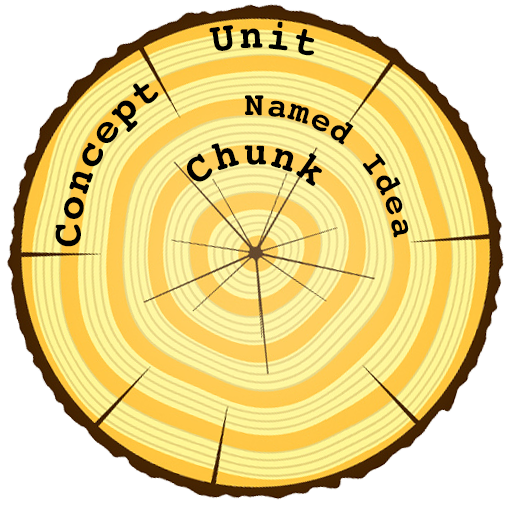
\includegraphics[scale=0.45]{Tree_Chunk_Model.png}
\end{frame}

\begin{frame}
\frametitle{Chunk Combinations}
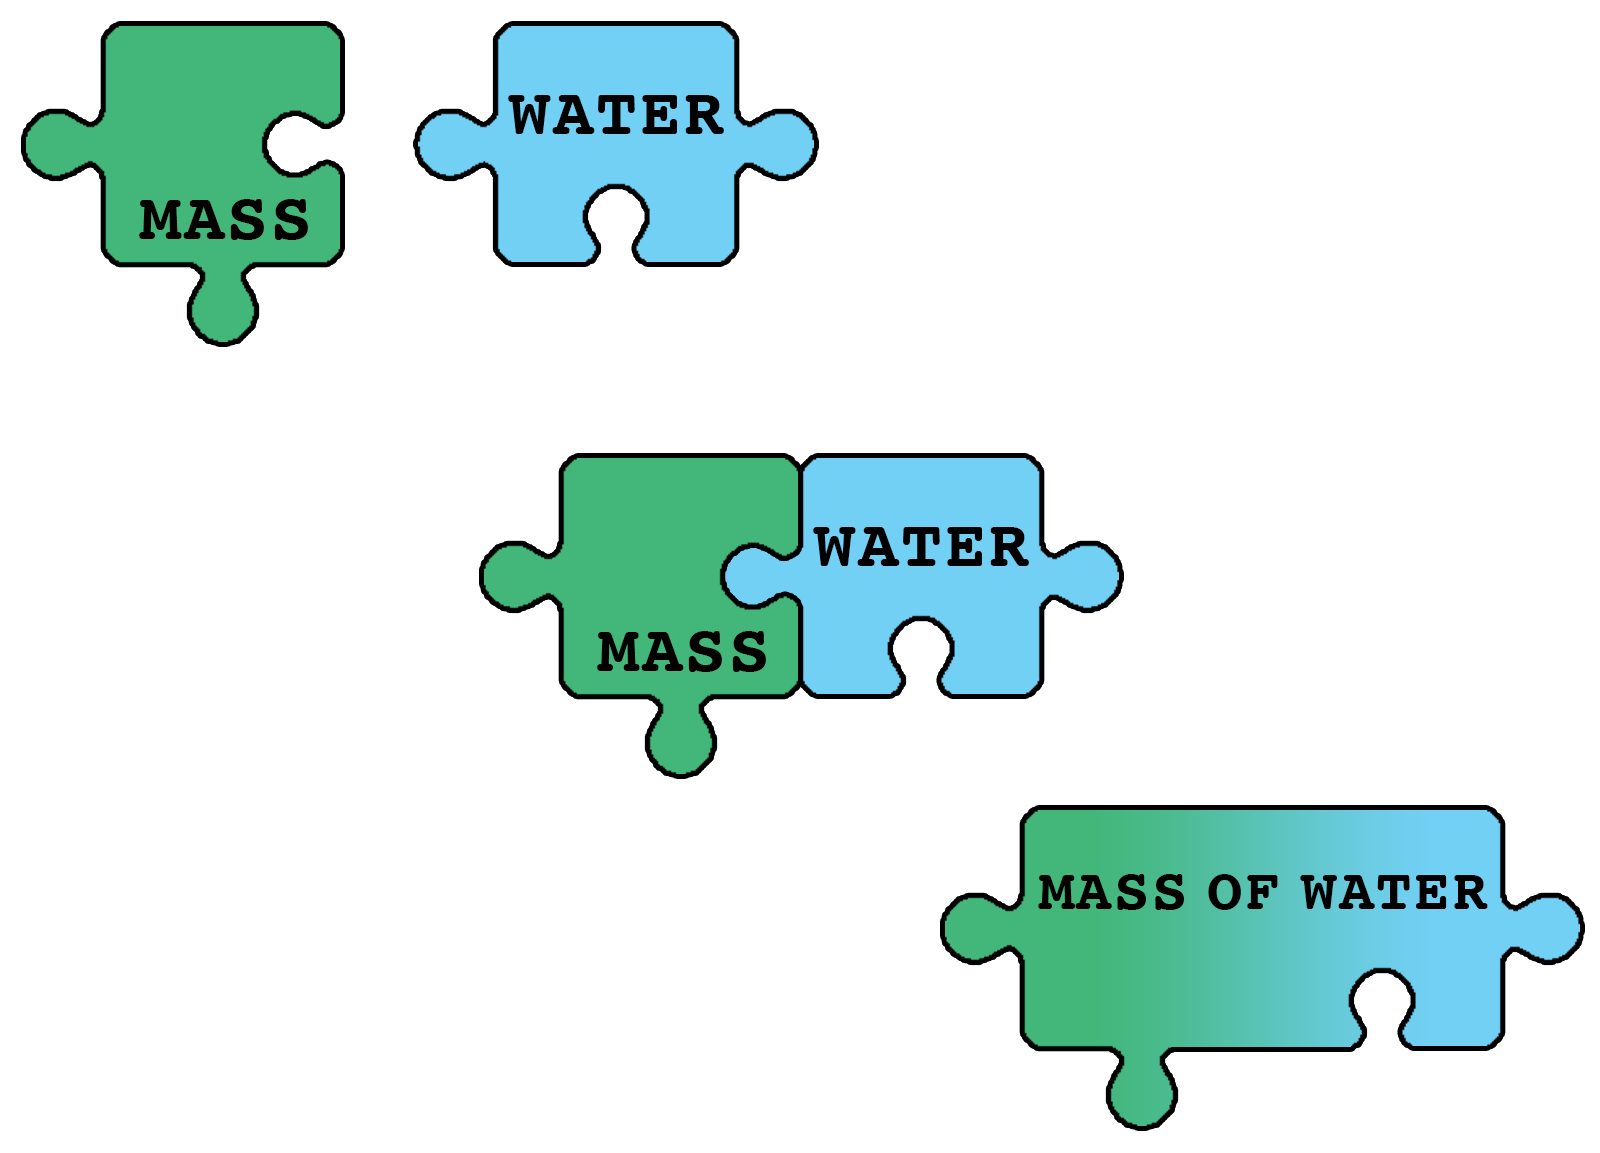
\includegraphics[scale=0.19]{Puzzle.png}
\end{frame}

\begin{frame}
\frametitle{Drasil Logic Tree}
\centering
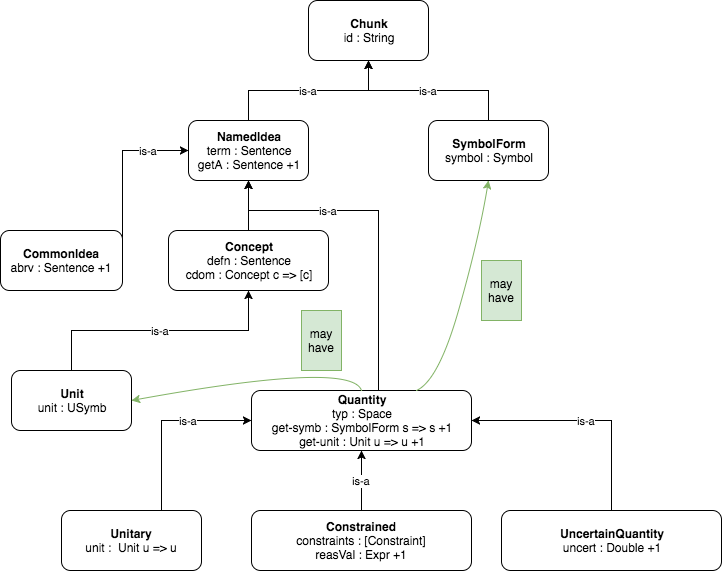
\includegraphics[scale=0.38]{../WG2_11/class_hierarchy.png}

\end{frame}

\begin{frame}
\frametitle{Collaborative Efforts}
\begin{itemize}
 \item<1-> Peer review of code\linebreak
 \item<2-> Discussion of all around issues (ex. cyclic imports, referencing problems)\linebreak
 \item<3-> A lot of collaboration through GitHub\linebreak
\end{itemize}
\end{frame}

\begin{frame}
\frametitle{Collaboration via Github}
\centering

\includegraphics[scale=0.2]{./Github_Logo.png}
\end{frame}

\begin{frame}
\frametitle{Collaboration via Github}
Git is a version control system, GitHub is a Git repository hosting service that is \alert{free}.
\begin{itemize}
 \item<1-> Git allows us to collaborate effectively, even when team members are not in the same location
\end{itemize}
\end{frame}

\begin{frame}
\frametitle{GitHub Issues}
\begin{center}
 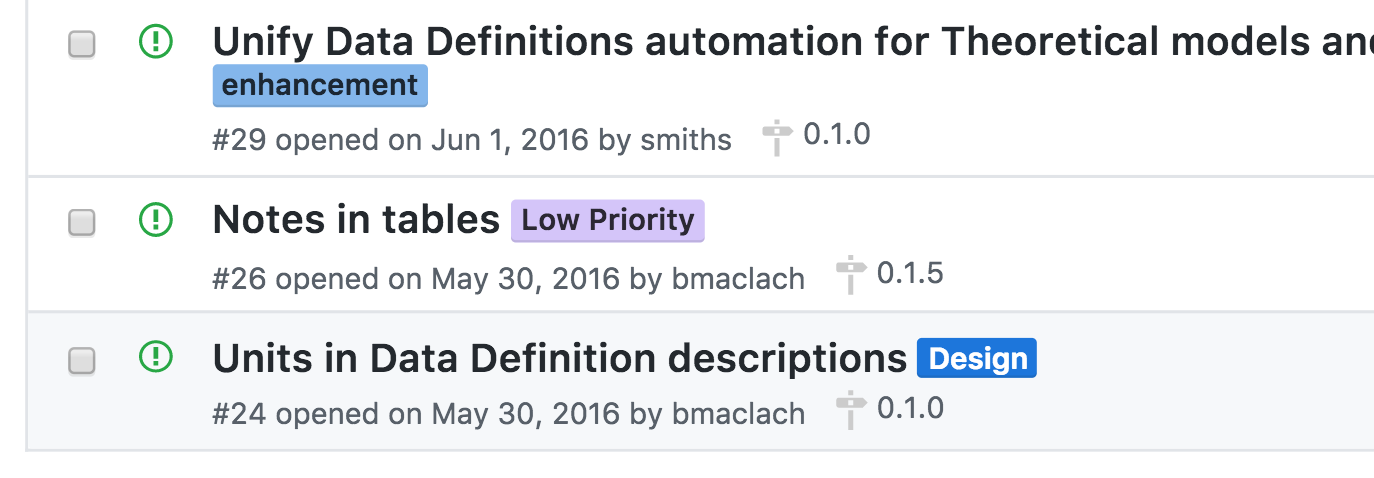
\includegraphics[scale=0.6]{Old_Issue.png}
\end{center}
\end{frame}

\begin{frame}
\frametitle{GitHub Issues}
\begin{center}
 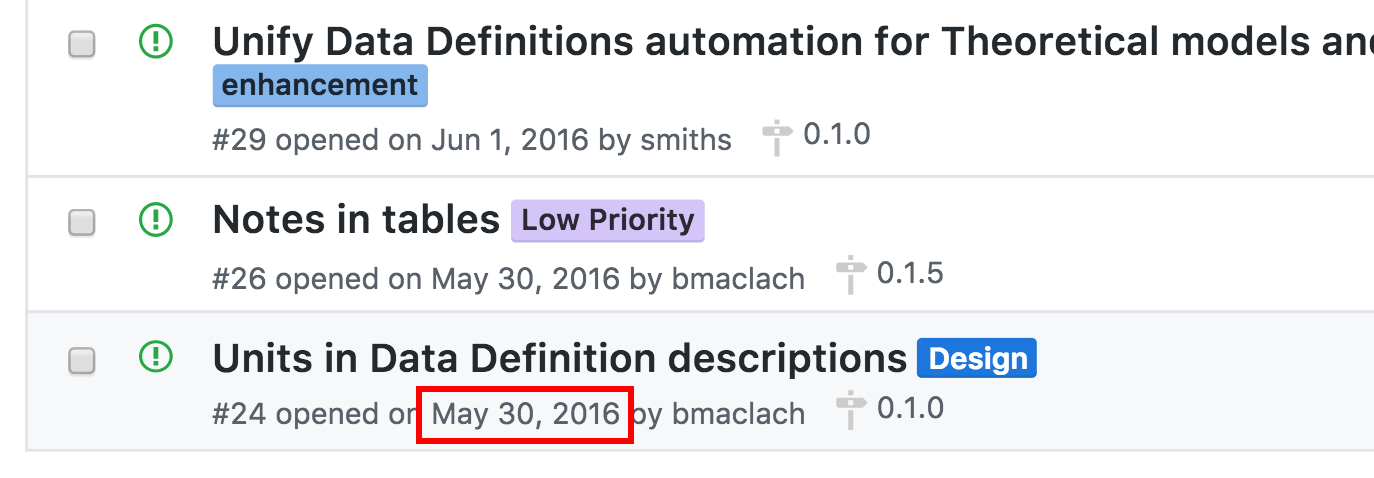
\includegraphics[scale=0.6]{Old_Issue_With_Box.png}
\end{center}
\end{frame}

\begin{frame}
\frametitle{Collaboration via Github}
Git is a version control system, GitHub is a Git repository hosting service that is \alert{free}.
\begin{itemize}
 \item<1-> Git allows us to collaborate effectively, even when team members are not in the same location
 \item<2-> Git combined with haskell, allows us to make large changes while easily maintaining a working version of Drasil
 \item<3-> Git \alert{(when used properly)} prevents catastrophic lose of work
\end{itemize}
\end{frame}

\begin{frame}
\frametitle{Daily Tasks}
\begin{itemize}
 \item<1-> Finding patterns within examples $\Rightarrow$ sentence combinators
 \item<1-> Finding patterns between examples $\Rightarrow$ extraction of common sections, contents, and concepts
 \begin{center}
  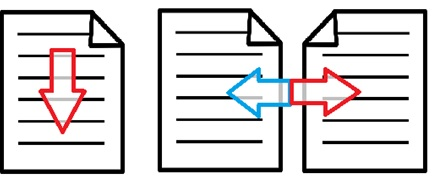
\includegraphics[scale=0.6]{WinAndBwExamples.jpg}
 \end{center}
 \item<2-> Knowledge extraction
 \item<2-> Reduced duplication due to
  \begin{itemize}
   \item Increased function efficiency
   \item Building chunks off of each other instead of from scratch
  \end{itemize}
\end{itemize}
\end{frame}

\begin{frame}
\frametitle{Example}
\centering
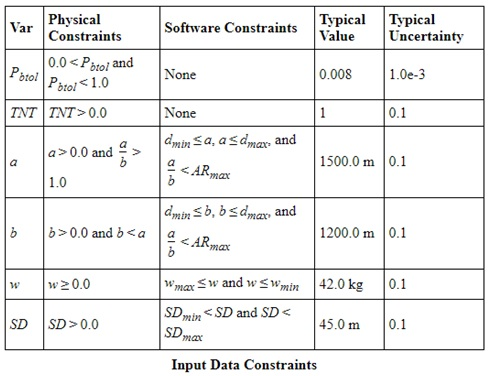
\includegraphics[scale=0.7]{InDataConsEx.jpg}
\end{frame}

\begin{frame}
\frametitle{Example}
\centering
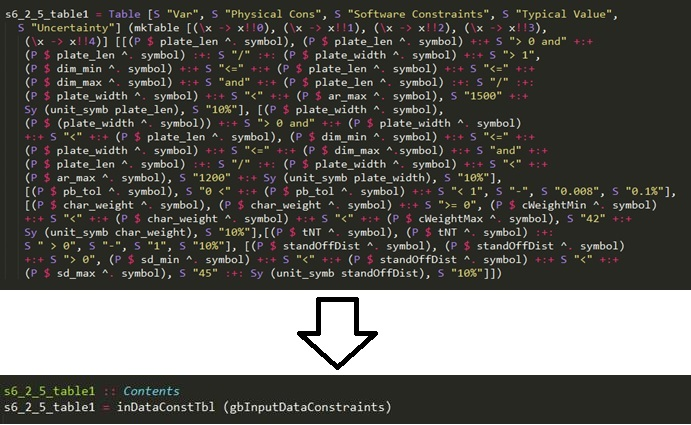
\includegraphics[scale=0.6]{CodeComparisons.jpg}
\end{frame}

\begin{frame}
\frametitle{Example}
\centering
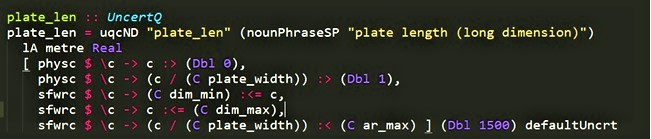
\includegraphics[height=0.25\textheight]{ChunkEx.jpg}
\newline
\newline
\newline
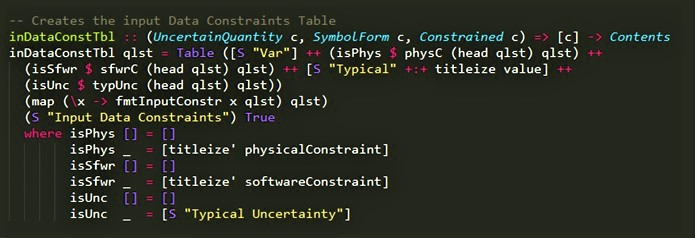
\includegraphics[height=0.40\textheight]{inDataConstTbl.jpg}
\end{frame}

\begin{frame}
\frametitle{Daily Tasks}
\begin{itemize}
 \item Finding patterns within examples $\Rightarrow$ sentence combinators
 \item Finding patterns between examples $\Rightarrow$ extraction of common sections, contents, and concepts
 \begin{center}
  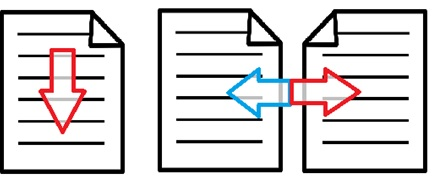
\includegraphics[scale=0.6]{WinAndBwExamples.jpg}
 \end{center}
 \item Knowledge extraction
 \item Reduced duplication due to
  \begin{itemize}
   \item Increased function efficiency
   \item Building chunks off of each other instead of from scratch
  \end{itemize}
 \item<1-> Implement new functions/types created by supervisors
 \item<2-> Code cleanup and bug fixing
 \item<3-> Opening/closing issues
\end{itemize}
\end{frame}

\begin{frame}
\frametitle{Case Study Contributions}
\begin{itemize}
\item Each member is assigned a case study as well as tasks and issues\newline
\item<1-> SWHS\newline
  \begin{itemize}
    \item Largest Example\newline
    \item ODEs\newline
  \end{itemize}
\item<2-> NoPCM\newline
  \begin{itemize}
    \item Builds off of pre-existing SWHS example\newline
  \end{itemize}
\item<3-> GlassBR\newline
  \begin{itemize}
    \item Omitted general definitions\newline
  \end{itemize}
\end{itemize}
\end{frame}

\begin{frame}
\frametitle{Case Study Contributions}
\begin{itemize}
\item<1-> SSP\newline
  \begin{itemize}
    \item Indexing\newline
    \item Sophisticated math\newline
    \item Diversity of symbols\newline
  \end{itemize}
\item<2-> GamePhysics\newline
  \begin{itemize}
    \item Most ambiguous example\newline
    \item SRS for a game physics library\newline
  \end{itemize}
\end{itemize}
\end{frame}

\begin{frame}
\frametitle{Future Improvements}
\begin{itemize}
 \item<1-> Still a lot more work to be done\newline
 \item<2-> ``Currently in a state of ordered chaos''\newline
 \item<3-> Code generation (recorded info $\Rightarrow$ useable code)\newline
 \item<4-> Proper referencing abilities\newline
 \item<5-> Complete auto generation of Table Of Symbols based on inputs\newline
 \item<6-> Identification of other word classes (ex. verbs, adjectives) and synonyms
\end{itemize}
\end{frame}

\begin{frame}
\frametitle{End}
For more information about Drasil and LLS visit our github page: \\
https://github.com/JacquesCarette/literate-scientific-software \\
\alert{You can even build a working version yourself!}
\newline
\newline
\begin{center}

\includegraphics[scale=0.5]{../WG2_11/generate_all_the_things.jpg}
\end{center}
\end{frame}

\end{document}